\documentclass[french]{book}
\usepackage[utf8x]{inputenc}
\usepackage[T1]{fontenc}
\usepackage{babel}
\usepackage{lmodern}
\usepackage[top=2cm,bottom=2cm,left=3cm,right=3cm]{geometry}
\usepackage{microtype}
\usepackage{mathtools, amssymb, amsthm}
\usepackage{mdframed}
\usepackage{hyperref}
\usepackage{graphicx}
\usepackage{xcolor}
\usepackage{mathrsfs}
\usepackage{wrapfig}
\usepackage{stmaryrd}
\usepackage{dsfont}
\usepackage{framed}
\usepackage{marginnote}
\usepackage[Glenn]{fncychap}

\theoremstyle{definition}
\newtheorem{prototheorem}{Théorème}[section]
\newenvironment{thm}
   {\colorlet{shadecolor}{orange!10}\begin{shaded}\begin{prototheorem}}
   {\end{prototheorem}\end{shaded}}

\newtheorem*{protocorollary}{Corollaire}
\newenvironment{corollary}
    {\colorlet{shadecolor}{violet!10}\begin{shaded}\begin{protocorollary}}
    {\end{protocorollary}\end{shaded}}

\newtheorem*{protolemma}{Lemme}
\newenvironment{lemma}
    {\colorlet{shadecolor}{pink!15}\begin{shaded}\begin{protolemma}}
    {\end{protolemma}\end{shaded}}


\newtheorem{protodefinition}{Définition}[section]
\newenvironment{definition}
    {\colorlet{shadecolor}{green!5}\begin{shaded}\begin{protodefinition}}
    {\end{protodefinition}\end{shaded}}

\newtheorem{protoproposition}{Proposition}[section]
\newenvironment{prop}
    {\colorlet{shadecolor}{blue!5}\begin{shaded}\begin{protoproposition}}
    {\end{protoproposition}\end{shaded}}

\newtheorem{protoremark}{Remarque}[section]
\newenvironment{remark}
    {\colorlet{shadecolor}{yellow!5}\begin{shaded}\begin{protoremark}}
    {\end{protoremark}\end{shaded}}

\newtheorem{exo}{Exercice}
\newtheorem*{protoexemple}{Exemple}
\newenvironment{exemple}
    {\colorlet{shadecolor}{gray!10}\begin{shaded}\begin{protoexemple}}
    {\end{protoexemple}\end{shaded}}


\newcommand{\less}{<}
\newcommand{\bg}{>}

\title{\bsc{Analyse fonctionnelle 2}}
\date{2023-2024}

\begin{document}

\maketitle

\tableofcontents

\chapter{Rappels et complements sur les EVN}

\section{Les séries dans les EVN} \marginnote{30-01-2024}

Soit \((E, \left\Vert \cdot \right\Vert )\) un EVN.

\begin{definition}
  On appelle \textbf{série de terme général} \(x_n\) dans \(E\) la suite \((S_n)_{n \in \mathbb{N}}\) telle que

  \[\forall n \in \mathbb{N}, S_n = \displaystyle\sum_{k=0}^{n} x_k, \text{ où } x_k \text{ est une suite d'éléments de } E.\]

  La série est convergente (cv) si la suite \((S_n)_{n \in \mathbb{N}}\) admet une limite dans \(E\).
\end{definition}

\begin{remark}
  En général on note \(\displaystyle\sum x_n\), la somme de la série est \(S = \displaystyle\sum_{k=0}^{+ \infty} x_n = \displaystyle\sum_{k \geq 0} x_n \).
\end{remark}

\begin{definition}
  La série \(\displaystyle\sum_{}^{}  x_n\) est dite \textbf{normalement convergente} si la série \(\displaystyle\sum_{}^{} \left\Vert x_n \right\Vert _{E}  \) est convergente dans \(\mathbb{R}^{+}\).
\end{definition}

\begin{thm}
  Soit \((E,\left\Vert \cdot \right\Vert )\) un espace de \textbf{\emph{Banach}}, alors toute série normalement convergente est convergente. De plus, on a

  \[\left\Vert \displaystyle\sum_{k=0}^{+\infty} x_n \right\Vert \leq \displaystyle\sum_{k=0}^{+\infty} \left\Vert x_n \right\Vert. \]
\end{thm}

\begin{proof}
  La série \(\displaystyle\sum_{}^{} \left\Vert x_n \right\Vert  \) est convergente dans \(\mathbb{R}\), donc de Cauchy : soit \(s_n = \displaystyle\sum_{k=0}^{n} \left\Vert x_n \right\Vert, n \in \mathbb{N}\) la somme partielle, alors

  \[\forall \varepsilon \bg 0, \exists N \text{ tel que } \forall p,q \geq  N, \text{  on a } \left\lvert s_p - s_q \right\rvert  = \displaystyle\sum_{k=p+1}^{q}\left\Vert x_k \right\Vert \leq \varepsilon. \]

  Dans ces conditions

  \begin{gather*}
    \left\Vert s_p - s_q \right\Vert = \left\Vert \displaystyle\sum_{k=p+1}^{q}   \right\Vert \leq \displaystyle\sum_{k=p+1}^{q} \left\Vert x_k \right\Vert  \leq  \varepsilon,
  \end{gather*}

  ce qui entraîne que \(S_n\) est de Cauchy dans \(E\). Mais \(E\) est complet, donc il existe \(S\) tel que \(\lim_{n \to \infty} S_n = S\).

  Mais par définition \(\lim_{n \to \infty} S_n = \displaystyle\sum_{k=0}^{+\infty} x_k = s \), donc elle est convergente.

  D'autre part, \(\forall n\), on a que

  \begin{gather*}
    \left\Vert \displaystyle\sum_{k=0}^{n} x_k  \right\Vert \leq  \displaystyle\sum_{k=0}^{n} \left\Vert x_k \right\Vert.
  \end{gather*}

  On a que \(\lim_{n \to \infty} \left\Vert \displaystyle\sum_{k=0}^{n}x_k  \right\Vert  = \left\Vert \lim_{n \to \infty} \displaystyle\sum_{k=0}^{n} x_k  \right\Vert = \left\Vert \displaystyle\sum_{k=0}^{+\infty} x_k  \right\Vert  \) (par continuité),
  et \(\lim_{n \to \infty} \displaystyle\sum_{k=0}^{n} \left\Vert x_k \right\Vert = \displaystyle\sum_{k=0}^{+\infty} \left\Vert x_k \right\Vert   \).

  Par passage à la limite, on obtient le résultat demandé.
\end{proof}

\section{Les espaces de Hilbert}

\begin{definition}

  \

  \begin{enumerate}
    \item Soit \(E\) un \(\mathbb{C}\)-espace. Une application \(\varphi : E \times E \longrightarrow \mathbb{C}\) est une \textbf{forme hermitienne} sur \(E\) si :

    \begin{enumerate}
      \item \(\forall y \in E\), \(x \in E \longmapsto \varphi(x,y)\) est linéaire ;
      \item \(\forall x,y \in E\), \(\varphi(x,y) = \overline{\varphi(y,x)}\).
    \end{enumerate}

    \item Un \textbf{produit scalaire} sur \(E\) est une forme hermitienne définie positive :

    \[\forall x \in E, \varphi(x,x) \geq  0 \text{ et } \varphi(x,x) = 0 \iff x=0_E.\]

    \item Un espace préhilbertien est un \(\mathbb{C}\)-espace muni d'un produit scalaire : \((E,\varphi)\).
  \end{enumerate}
\end{definition}

\begin{remark}
  \(\varphi(x,y) = (x \mid y)\).
\end{remark}

Comme conséquence : \(\forall x \in E\), \(\varphi ^{1/2}(x,x) = (x | x) ^{1/2}\) est une norme sur \(E\) (le vérifier en exercice).

\begin{prop}[Cauchy-Schwarz]
  On rappelle que l'on a

  \[\forall x,y \in E, \left\lvert (x | y) \right\rvert \leq \left\Vert x\right\Vert_E \left\Vert y \right\Vert_E\]

  et on a égalité dans le cas où \(x,y\) sont colinéaires.
\end{prop}

Un espace préhilbertien est un EVN, et donc un espace métrique avec la distance

\[\forall x,y \in E, d_E(x,y) = \left\Vert x-y \right\Vert_E = (x-y | x-y)_E ^{1/2}.\]

\begin{definition}
  Un espace de Hilbert est un espace préhilbertien complet.
\end{definition}

\begin{exo}
  Montrer que les applications suivantes sont continues :

  \begin{enumerate}
    \item \(\forall y \in E, x \in E \longmapsto (x | y)\) ;
    \item \(\forall x \in E, y \in E \longmapsto (x | y)\).
  \end{enumerate}
\end{exo}

\begin{definition}
  Deux vecteurs \(x,y \in E\) sont dits \textbf{orthogonaux} si \((x \mid y) = 0\) (on note aussi \(x \perp y\)).

  Plus généralement, soit \(A \subset E\), \(x \in E\) est orthogonal à \(A\) si

  \[\forall y \in A, (x | y) = 0\]

  ou encore si \(A,B \subset E\), \(A\) est orthogonal à \(B\) si

  \[\forall x \in A, \forall y \in B, (x \mid y) =0.\]

  En particulier, on notera par \(A ^{ \perp} = \{  x \in E, x \perp A\}\).
\end{definition}

\begin{exo}
  Montrer que \(\forall A \subset E, A ^{\perp}\) est un sous-espace vectoriel. Montrer aussi que \(A ^{\perp}\) est un sous-espace fermé de \(E\).
\end{exo}

\begin{figure}[h!]
  \centering
  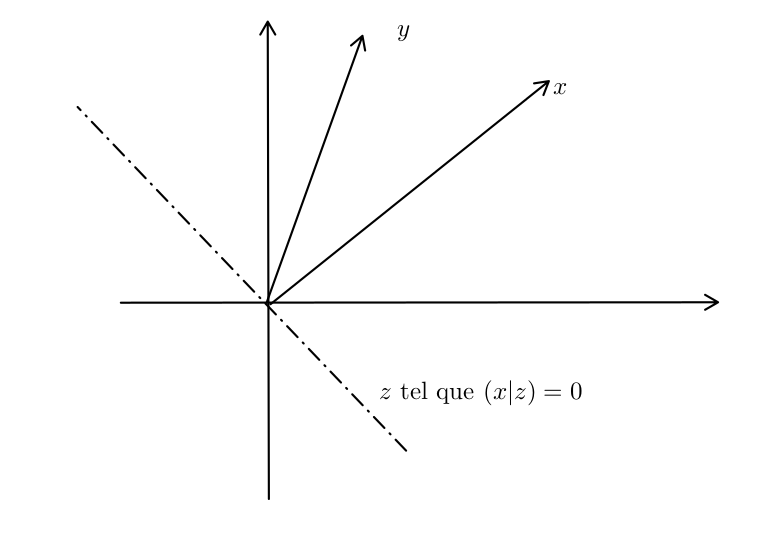
\includegraphics[scale=0.3]{figures/scal_r2.png}
  \caption{Le produit scalaire et les orthogonaux dans \(\mathbb{R}^2\).}
  \label{}
\end{figure}

\begin{exemple}
  Soit \(E = \mathbb{C}^{N}\), alors \(x,y \in E\), les composantes sont \(i \in 1, \dots, N\) telles que \(x(i) \in \mathbb{C}, y(i) \in \mathbb{C}\). On a le produit scalaire sur \(\mathbb{C}^{N}\) :

  \[(x \mid y) = \displaystyle\sum_{i=1}^{N} x(i)\overline{y(i)},\]

  on déduit la norme associée. Il satisfait l'inégalité de Cauchy-Schwarz :

  \[\left\lvert (x \mid y) \right\rvert = \left\lvert \displaystyle\sum_{i=1}^{N} x(i) \overline{y(i)} \right\rvert \leq \left\Vert x \right\Vert \left\Vert y \right\Vert =  \sqrt{\displaystyle\sum_{i=1}^{n} \left\lvert x(i) \right\rvert ^2 } \sqrt{\displaystyle\sum_{i=1}^{n} \left\lvert y(i) \right\rvert ^2 }.\]
\end{exemple}

\section{Théorème de la projection orthogonale}

Soit \(\mathcal{H}\) un espace de Hilbert. On rappelle que \(C \subset \mathcal{H}\) est convexe si \[\forall (x,y) \in \mathcal{H}\times \mathcal{H}, \lambda x + (1 - \lambda)y \in \mathcal{H}, \forall \lambda \in [0,1].\]


\begin{thm}
  Dans ces conditions, soit \(\mathbb{C}\) un convexe fermé non vide de \(\mathcal{H}\). Alors pour tout \(x \in \mathcal{H}\), il existe un unique point \(y_0 \in C\) tel que

  \[\operatorname{dist}(x,C) = \inf_{y \in C} \left\Vert x-y \right\Vert _{\mathcal{H}} = \left\Vert x - y_0 \right\Vert.\]

  et pour tout \(y \in \mathbb{C}\), \(\Re(x-y_0 \mid y - y_0) \leq 0\).

  \(y_0\) s'appelle la \textbf{projection orthogonale} de \(x\) sur \(\mathbb{C}\).
\end{thm}

\begin{figure}[h!]
  \centering
  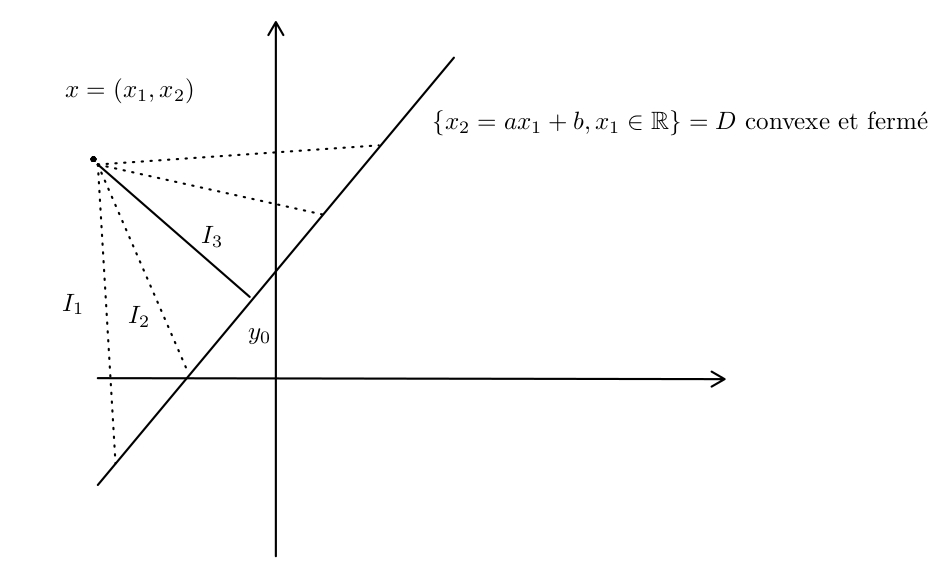
\includegraphics[scale=0.3]{figures/proj-ortho.png}
  \caption{Illustrtion du théorème de la projection orthogonale. \(I_3\) est la plus petite distance.}
  \label{}
\end{figure}

\begin{figure}[h!]
  \centering
  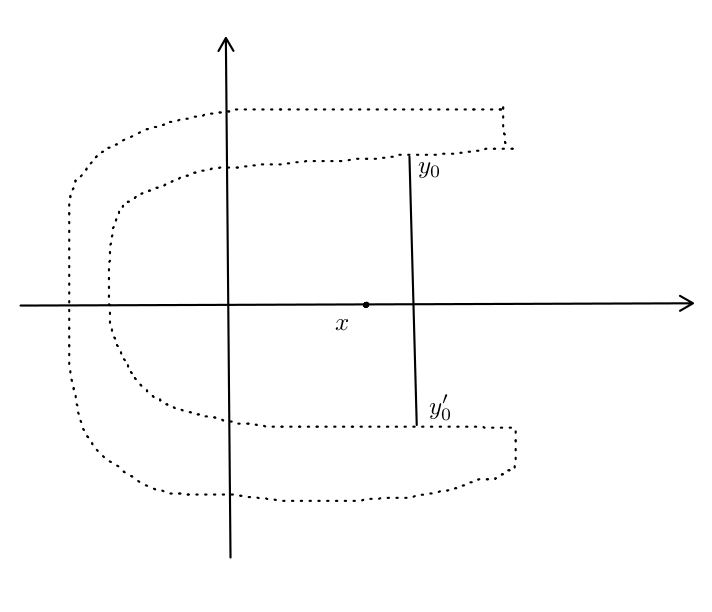
\includegraphics[scale=0.3]{figures/proj-ortho2.png}
  \caption{Deux projections orthogonales. L'unicité est contredite.}
  \label{}
\end{figure}

\begin{exo}
  Soit \(F\) un sous-espace fermé de \(\mathcal{H}\). Montrer que \(\mathcal{H} = F \oplus F ^{\perp}\).
\end{exo}

\begin{definition}
  Soit \(F\) un sous-espace fermé. On appelle \textbf{projection orthogonale} sur \(F\) l'application définie de la manière suivante : \(\forall x \in \mathcal{H}, x = x_1 + x_2, x_1 \in F, x_2 \in F ^{\perp}, x_1, x_2 \text{ uniques } \) :

  \[P_F x = x_1 (P _{F ^{\perp}} = x_2).\]
\end{definition}

\begin{prop}
  \(P_F : \mathcal{H} \longrightarrow \mathcal{H}\) est linéaire et continue.
\end{prop}

\begin{proof}
  On calcule :

  \[\left\Vert P_F x \right\Vert ^2 = (P_F x \mid P_F x) = (x_1 \mid x_1) = \left\Vert x_1 \right\Vert ^2 \leq \left\Vert x_1 \right\Vert ^2 + \left\Vert x_2 \right\Vert ^2 = \left\Vert x \right\Vert ^2.\]

  (théorème de Pythagore).

  On a donc \(\forall x \in \mathcal{H}, \left\Vert P_F x \right\Vert \leq \left\Vert x \right\Vert\).
\end{proof}

\begin{remark}
  Si \(x \in F\), alors la projection orthogonale est \(y_0 = x\).
\end{remark}

\begin{remark}
  Ici \(P_F x = x\), ce qui implique que \(\left\Vert P_F x \right\Vert  = \left\Vert x \right\Vert \leq \left\Vert P_F \right\Vert \left\Vert x \right\Vert \), donc \(\left\Vert P_F \right\Vert \geq 1 \) et donc \(\left\Vert P_F \right\Vert =1\).
\end{remark}

\begin{definition}
  Une partie \(A \subset \mathcal{H}\) est \textbf{totale} si le plus petit sous-espace fermé contenant \(A\) est \(\overline{\operatorname{vect}\{ A \}} = \mathcal{H}\).
\end{definition}


\begin{exo}
  De manière générale, si \(A \subset \mathcal{H}\), montrer que le plus petit sous-espace fermé contenant \(A\) est \((A ^{\perp})^{\perp} = A ^{\perp \perp}\). En déduire que \(A\) est totale si et seulement si \(A ^{\perp} = \{ 0 _{\mathcal{H}} \}\).
\end{exo}

\begin{definition}
  \(\mathcal{H}\) est \textbf{séparable} s'il admet une famille totale dénombrable.
\end{definition}

\begin{exo}
  Montrer que \(l ^2(\mathbb{N})\) est séparable.
\end{exo}

Dans ce cours, on considérera en général des espaces de Hilbert séparables.

\end{document}
